% Created 2021-07-06 Tue 16:13
% Intended LaTeX compiler: pdflatex
\documentclass[11pt]{article}
\usepackage[utf8]{inputenc}
\usepackage[T1]{fontenc}
\usepackage{graphicx}
\usepackage{grffile}
\usepackage{longtable}
\usepackage{wrapfig}
\usepackage{rotating}
\usepackage[normalem]{ulem}
\usepackage{amsmath}
\usepackage{textcomp}
\usepackage{amssymb}
\usepackage{capt-of}
\usepackage{hyperref}
\graphicspath{{../../books/}}
%%%%%%%%%%%%%%%%%%%%%%%%%%%%%%%%%%%%%%
%% TIPS                                 %%
%%%%%%%%%%%%%%%%%%%%%%%%%%%%%%%%%%%%%%
% \substack{a\\b} for multiple lines text

\usepackage[utf8]{inputenc}

\usepackage[B1,T1]{fontenc}

% pdfplots will load xolor automatically without option
\usepackage[dvipsnames]{xcolor}
%%%%%%%%%%%%%%%%%%%%%%%%%%%%%%%%%%%%%%%
%% MATH related pacakge                  %%
%%%%%%%%%%%%%%%%%%%%%%%%%%%%%%%%%%%%%%%
% \usepackage{amsmath} mathtools loads the amsmath
\usepackage{amsmath}
\usepackage{mathtools}


\usepackage{amsthm}
\usepackage{amsbsy}

%\usepackage{commath}

\usepackage{amssymb}
\usepackage{mathrsfs}
%\usepackage{mathabx}
\usepackage{stmaryrd}
\usepackage{empheq}

%for \not\ll
\usepackage{centernot}

\usepackage{scalerel}
\usepackage{stackengine}
\usepackage{stackrel}

\usepackage{nicematrix}
\usepackage{tensor}
\usepackage{blkarray}
\usepackage{siunitx}
\usepackage[f]{esvect}

\usepackage{unicode-math}
\setmainfont{TeX Gyre Pagella}
% \setmathfont{STIX}
%\setmathfont{texgyrepagella-math.otf}
%\setmathfont{Libertinus Math}
\setmathfont{Latin Modern Math}

 
% \setmathfont[range={\smwhtdiamond,\enclosediamond,\varlrtriangle}]{Latin Modern Math}
 \setmathfont[range={\rightrightarrows,\twoheadrightarrow,\leftrightsquigarrow,\triangledown,\vartriangle}]{XITS Math}
 \setmathfont[range={\int,\setminus}]{Libertinus Math}
 \setmathfont[range={\mathalpha}]{TeX Gyre Pagella Math}
% unicode is not good at this!
%\let\nmodels\nvDash


%%%%%%%%%%%%%%%%%%%%%%%%%%%%%%%%%%%%%%%
%% TIKZ related packages                 %%
%%%%%%%%%%%%%%%%%%%%%%%%%%%%%%%%%%%%%%%

\usepackage{pgfplots}
\pgfplotsset{compat=1.15}
\usepackage{tikz}
\usepackage{tikz-cd}
\usepackage{tikz-qtree}

\usetikzlibrary{arrows,positioning,calc,fadings,decorations,matrix,decorations,shapes.misc}
%setting from geogebra
\definecolor{ccqqqq}{rgb}{0.8,0,0}


%%%%%%%%%%%%%%%%%%%%%%%%%%%%%%%%%%%%%%%
%% MISCLELLANEOUS packages               %%
%%%%%%%%%%%%%%%%%%%%%%%%%%%%%%%%%%%%%%%
\usepackage[most]{tcolorbox}
\usepackage{threeparttable}
\usepackage{tabularx}

\usepackage{enumitem}

% wrong with preview
\usepackage{subcaption}
\usepackage{caption}
% {\aunclfamily\Huge}
\usepackage{auncial}

\usepackage{float}

\usepackage{fancyhdr}

\usepackage{ifthen}
\usepackage{xargs}


\usepackage{imakeidx}
\usepackage{hyperref}
\usepackage{soul}


%\usepackage[xetex]{preview}
%%%%%%%%%%%%%%%%%%%%%%%%%%%%%%%%%%%%%%%
%% USEPACKAGES end                       %%
%%%%%%%%%%%%%%%%%%%%%%%%%%%%%%%%%%%%%%%

% \setlist{nosep}
% \numberwithin{equation}{subsection}
% \fancyhead{} % Clear the headers
% \renewcommand{\headrulewidth}{0pt} % Width of line at top of page
% \fancyhead[R]{\slshape\leftmark} % Mark right [R] of page with Chapter name [\leftmark]
% \pagestyle{fancy} % Set default style for all content pages (not TOC, etc)


% \newlength\shlength
% \newcommand\vect[2][0]{\setlength\shlength{#1pt}%
%   \stackengine{-5.6pt}{$#2$}{\smash{$\kern\shlength%
%     \stackengine{7.55pt}{$\mathchar"017E$}%
%       {\rule{\widthof{$#2$}}{.57pt}\kern.4pt}{O}{r}{F}{F}{L}\kern-\shlength$}}%
%       {O}{c}{F}{T}{S}}


\indexsetup{othercode=\small}
\makeindex[columns=2,options={-s /media/wu/file/stuuudy/notes/index_style.ist},intoc]
\makeatletter
\def\@idxitem{\par\hangindent 0pt}
\makeatother


%\newcounter{dummy} \numberwithin{dummy}{section}
\newtheorem{dummy}{dummy}[section]
\theoremstyle{definition}
\newtheorem{definition}[dummy]{Definition}
\theoremstyle{plain}
\newtheorem{corollary}[dummy]{Corollary}
\newtheorem{lemma}[dummy]{Lemma}
\newtheorem{proposition}[dummy]{Proposition}
\newtheorem{theorem}[dummy]{Theorem}
\theoremstyle{definition}
\newtheorem{examplle}{Example}[section]
\theoremstyle{remark}
\newtheorem*{remark}{Remark}
\newtheorem{exercise}{Exercise}[subsection]
\newtheorem{observation}{Observation}[section]


\newenvironment{claim}[1]{\par\noindent\textbf{Claim:}\space#1}{}

\makeatletter
\DeclareFontFamily{U}{tipa}{}
\DeclareFontShape{U}{tipa}{m}{n}{<->tipa10}{}
\newcommand{\arc@char}{{\usefont{U}{tipa}{m}{n}\symbol{62}}}%

\newcommand{\arc}[1]{\mathpalette\arc@arc{#1}}

\newcommand{\arc@arc}[2]{%
  \sbox0{$\m@th#1#2$}%
  \vbox{
    \hbox{\resizebox{\wd0}{\height}{\arc@char}}
    \nointerlineskip
    \box0
  }%
}
\makeatother

\setcounter{MaxMatrixCols}{20}
%%%%%%% ABS
\DeclarePairedDelimiter\abss{\lvert}{\rvert}%
\DeclarePairedDelimiter\normm{\lVert}{\rVert}%

% Swap the definition of \abs* and \norm*, so that \abs
% and \norm resizes the size of the brackets, and the
% starred version does not.
\makeatletter
\let\oldabs\abss
%\def\abs{\@ifstar{\oldabs}{\oldabs*}}
\newcommand{\abs}{\@ifstar{\oldabs}{\oldabs*}}
\newcommand{\norm}[1]{\left\lVert#1\right\rVert}
%\let\oldnorm\normm
%\def\norm{\@ifstar{\oldnorm}{\oldnorm*}}
%\renewcommand{norm}{\@ifstar{\oldnorm}{\oldnorm*}}
\makeatother

% \newcommand\what[1]{\ThisStyle{%
%     \setbox0=\hbox{$\SavedStyle#1$}%
%     \stackengine{-1.0\ht0+.5pt}{$\SavedStyle#1$}{%
%       \stretchto{\scaleto{\SavedStyle\mkern.15mu\char'136}{2.6\wd0}}{1.4\ht0}%
%     }{O}{c}{F}{T}{S}%
%   }
% }

% \newcommand\wtilde[1]{\ThisStyle{%
%     \setbox0=\hbox{$\SavedStyle#1$}%
%     \stackengine{-.1\LMpt}{$\SavedStyle#1$}{%
%       \stretchto{\scaleto{\SavedStyle\mkern.2mu\AC}{.5150\wd0}}{.6\ht0}%
%     }{O}{c}{F}{T}{S}%
%   }
% }

% \newcommand\wbar[1]{\ThisStyle{%
%     \setbox0=\hbox{$\SavedStyle#1$}%
%     \stackengine{.5pt+\LMpt}{$\SavedStyle#1$}{%
%       \rule{\wd0}{\dimexpr.3\LMpt+.3pt}%
%     }{O}{c}{F}{T}{S}%
%   }
% }

\newcommand{\bl}[1] {\boldsymbol{#1}}
\newcommand{\Wt}[1] {\stackrel{\sim}{\smash{#1}\rule{0pt}{1.1ex}}}
\newcommand{\wt}[1] {\widetilde{#1}}
\newcommand{\tf}[1] {\textbf{#1}}


%For boxed texts in align, use Aboxed{}
%otherwise use boxed{}

\DeclareMathSymbol{\widehatsym}{\mathord}{largesymbols}{"62}
\newcommand\lowerwidehatsym{%
  \text{\smash{\raisebox{-1.3ex}{%
    $\widehatsym$}}}}
\newcommand\fixwidehat[1]{%
  \mathchoice
    {\accentset{\displaystyle\lowerwidehatsym}{#1}}
    {\accentset{\textstyle\lowerwidehatsym}{#1}}
    {\accentset{\scriptstyle\lowerwidehatsym}{#1}}
    {\accentset{\scriptscriptstyle\lowerwidehatsym}{#1}}
  }


\newcommand{\cupdot}{\mathbin{\dot{\cup}}}
\newcommand{\bigcupdot}{\mathop{\dot{\bigcup}}}

\usepackage{graphicx}

\usepackage[toc,page]{appendix}

% text on arrow for xRightarrow
\makeatletter
%\newcommand{\xRightarrow}[2][]{\ext@arrow 0359\Rightarrowfill@{#1}{#2}}
\makeatother

% Arbitrary long arrow
\newcommand{\Rarrow}[1]{%
\parbox{#1}{\tikz{\draw[->](0,0)--(#1,0);}}
}

\newcommand{\LRarrow}[1]{%
\parbox{#1}{\tikz{\draw[<->](0,0)--(#1,0);}}
}


\makeatletter
\providecommand*{\rmodels}{%
  \mathrel{%
    \mathpalette\@rmodels\models
  }%
}
\newcommand*{\@rmodels}[2]{%
  \reflectbox{$\m@th#1#2$}%
}
\makeatother







\newcommand{\trcl}[1]{%
  \mathrm{trcl}{(#1)}
}



% Roman numerals
\makeatletter
\newcommand*{\rom}[1]{\expandafter\@slowromancap\romannumeral #1@}
\makeatother
% \\def \\b\([a-zA-Z]\) {\\boldsymbol{[a-zA-z]}}
% \\DeclareMathOperator{\\b\1}{\\textbf{\1}}


\DeclareMathOperator{\bx}{\textbf{x}}
\DeclareMathOperator{\bz}{\textbf{z}}
\DeclareMathOperator{\bff}{\textbf{f}}
\DeclareMathOperator{\ba}{\textbf{a}}
\DeclareMathOperator{\bk}{\textbf{k}}
\DeclareMathOperator{\bs}{\textbf{s}}
\DeclareMathOperator{\bh}{\textbf{h}}
\DeclareMathOperator{\bc}{\textbf{c}}
\DeclareMathOperator{\br}{\textbf{r}}
\DeclareMathOperator{\bi}{\textbf{i}}
\DeclareMathOperator{\bj}{\textbf{j}}
\DeclareMathOperator{\bn}{\textbf{n}}
\DeclareMathOperator{\be}{\textbf{e}}
\DeclareMathOperator{\bo}{\textbf{o}}
\DeclareMathOperator{\bU}{\textbf{U}}
\DeclareMathOperator{\bL}{\textbf{L}}
\DeclareMathOperator{\bV}{\textbf{V}}
\def \bzero {\mathbf{0}}
\def \btwo {\mathbf{2}}
\DeclareMathOperator{\bv}{\textbf{v}}
\DeclareMathOperator{\bp}{\textbf{p}}
\DeclareMathOperator{\bI}{\textbf{I}}
\DeclareMathOperator{\bM}{\textbf{M}}
\DeclareMathOperator{\bN}{\textbf{N}}
\DeclareMathOperator{\bK}{\textbf{K}}
\DeclareMathOperator{\bt}{\textbf{t}}
\DeclareMathOperator{\bb}{\textbf{b}}
\DeclareMathOperator{\bA}{\textbf{A}}
\DeclareMathOperator{\bX}{\textbf{X}}
\DeclareMathOperator{\bu}{\textbf{u}}
\DeclareMathOperator{\bS}{\textbf{S}}
\DeclareMathOperator{\bZ}{\textbf{Z}}
\DeclareMathOperator{\bJ}{\textbf{J}}
\DeclareMathOperator{\by}{\textbf{y}}
\DeclareMathOperator{\bw}{\textbf{w}}
\DeclareMathOperator{\bT}{\textbf{T}}
\DeclareMathOperator{\bF}{\textbf{F}}
\DeclareMathOperator{\bmm}{\textbf{m}}
\DeclareMathOperator{\bW}{\textbf{W}}
\DeclareMathOperator{\bR}{\textbf{R}}
\DeclareMathOperator{\bC}{\textbf{C}}
\DeclareMathOperator{\bD}{\textbf{D}}
\DeclareMathOperator{\bE}{\textbf{E}}
\DeclareMathOperator{\bQ}{\textbf{Q}}
\DeclareMathOperator{\bP}{\textbf{P}}
\DeclareMathOperator{\bY}{\textbf{Y}}
\DeclareMathOperator{\bH}{\textbf{H}}
\DeclareMathOperator{\bB}{\textbf{B}}
\DeclareMathOperator{\bG}{\textbf{G}}
\def \blambda {\symbf{\lambda}}
\def \boldeta {\symbf{\eta}}
\def \balpha {\symbf{\alpha}}
\def \bbeta {\symbf{\beta}}
\def \bgamma {\symbf{\gamma}}
\def \bxi {\symbf{\xi}}
\def \bLambda {\symbf{\Lambda}}
\def \bGamma {\symbf{\Gamma}}

\newcommand{\bto}{{\boldsymbol{\to}}}
\newcommand{\Ra}{\Rightarrow}
\newcommand\und[1]{\underline{#1}}
\newcommand\ove[1]{\overline{#1}}
\def \bPhi {\boldsymbol{\Phi}}
\def \btheta {\boldsymbol{\theta}}
\def \bTheta {\boldsymbol{\Theta}}
\def \bmu {\boldsymbol{\mu}}
\def \bphi {\boldsymbol{\phi}}
\def \bSigma {\boldsymbol{\Sigma}}
\def \lb {\left\{}
\def \rb {\right\}}
\def \la {\langle}
\def \ra {\rangle}
\def \caln {\mathcal{N}}
\def \dissum {\displaystyle\Sigma}
\def \dispro {\displaystyle\prod}
\def \E {\mathbb{E}}
\def \Q {\mathbb{Q}}
\def \N {\mathbb{N}}
\def \V {\mathbb{V}}
\def \R {\mathbb{R}}
\def \P {\mathbb{P}}
\def \A {\mathbb{A}}
\def \F {\mathbb{F}}
\def \Z {\mathbb{Z}}
\def \I {\mathbb{I}}
\def \C {\mathbb{C}}
\def \cala {\mathcal{A}}
\def \cale {\mathcal{E}}
\def \calb {\mathcal{B}}
\def \calq {\mathcal{Q}}
\def \calp {\mathcal{P}}
\def \cals {\mathcal{S}}
\def \calx {\mathcal{X}}
\def \caly {\mathcal{Y}}
\def \calg {\mathcal{G}}
\def \cald {\mathcal{D}}
\def \caln {\mathcal{N}}
\def \calr {\mathcal{R}}
\def \calt {\mathcal{T}}
\def \calm {\mathcal{M}}
\def \calw {\mathcal{W}}
\def \calc {\mathcal{C}}
\def \calv {\mathcal{V}}
\def \calf {\mathcal{F}}
\def \calk {\mathcal{K}}
\def \call {\mathcal{L}}
\def \calu {\mathcal{U}}
\def \calo {\mathcal{O}}
\def \calh {\mathcal{H}}
\def \cali {\mathcal{I}}

\def \bcup {\bigcup}

% set theory

\def \zfcc {\textbf{ZFC}^-}
\def \ac  {\textbf{AC}}
\def \gl  {\textbf{L }}
\def \gll {\textbf{L}}
\newcommand{\zfm}{$\textbf{ZF}^-$}

%\def \zfm {$\textbf{ZF}^-$}
\def \zfmm {\textbf{ZF}^-}
\def \wf {\textbf{WF }}
\def \on {\textbf{On }}
\def \cm {\textbf{M }}
\def \cn {\textbf{N }}
\def \cv {\textbf{V }}
\def \zc {\textbf{ZC }}
\def \zcm {\textbf{ZC}}
\def \zff {\textbf{ZF}}
\def \wfm {\textbf{WF}}
\def \onm {\textbf{On}}
\def \cmm {\textbf{M}}
\def \cnm {\textbf{N}}
\def \cvm {\textbf{V}}
\def \gchh {\textbf{GCH}}
\renewcommand{\restriction}{\mathord{\upharpoonright}}
\def \pred {\text{pred}}

\def \rank {\text{rank}}
\def \con {\text{Con}}
\def \deff {\text{Def}}


\def \uin {\underline{\in}}
\def \oin {\overline{\in}}
\def \uR {\underline{R}}
\def \oR {\overline{R}}
\def \uP {\underline{P}}
\def \oP {\overline{P}}

\def \dsum {\displaystyle\sum}

\def \Ra {\Rightarrow}

\def \e {\enspace}

\def \sgn {\operatorname{sgn}}
\def \gen {\operatorname{gen}}
\def \Hom {\operatorname{Hom}}
\def \hom {\operatorname{hom}}
\def \Sub {\operatorname{Sub}}

\def \supp {\operatorname{supp}}

\def \epiarrow {\twoheadarrow}
\def \monoarrow {\rightarrowtail}
\def \rrarrow {\rightrightarrows}

% \def \minus {\text{-}}
% \newcommand{\minus}{\scalebox{0.75}[1.0]{$-$}}
% \DeclareUnicodeCharacter{002D}{\minus}


\def \tril {\triangleleft}

\def \ACF {\text{ACF}}
\def \GL {\text{GL}}
\def \PGL {\text{PGL}}
\def \equal {=}
\def \deg {\text{deg}}
\def \degree {\text{degree}}
\def \app {\text{App}}
\def \FV {\text{FV}}
\def \conv {\text{conv}}
\def \cont {\text{cont}}
\DeclareMathOperator{\cl}{\textbf{CL}}
\DeclareMathOperator{\sg}{sg}
\DeclareMathOperator{\trdeg}{trdeg}
\def \Ord {\text{Ord}}

\DeclareMathOperator{\cf}{cf}
\DeclareMathOperator{\zfc}{ZFC}

%\DeclareMathOperator{\Th}{Th}
%\def \th {\text{Th}}
% \newcommand{\th}{\text{Th}}
\DeclareMathOperator{\type}{type}
\DeclareMathOperator{\zf}{\textbf{ZF}}
\def \fa {\mathfrak{a}}
\def \fb {\mathfrak{b}}
\def \fc {\mathfrak{c}}
\def \fd {\mathfrak{d}}
\def \fe {\mathfrak{e}}
\def \ff {\mathfrak{f}}
\def \fg {\mathfrak{g}}
\def \fh {\mathfrak{h}}
%\def \fi {\mathfrak{i}}
\def \fj {\mathfrak{j}}
\def \fk {\mathfrak{k}}
\def \fl {\mathfrak{l}}
\def \fm {\mathfrak{m}}
\def \fn {\mathfrak{n}}
\def \fo {\mathfrak{o}}
\def \fp {\mathfrak{p}}
\def \fq {\mathfrak{q}}
\def \fr {\mathfrak{r}}
\def \fs {\mathfrak{s}}
\def \ft {\mathfrak{t}}
\def \fu {\mathfrak{u}}
\def \fv {\mathfrak{v}}
\def \fw {\mathfrak{w}}
\def \fx {\mathfrak{x}}
\def \fy {\mathfrak{y}}
\def \fz {\mathfrak{z}}
\def \fA {\mathfrak{A}}
\def \fB {\mathfrak{B}}
\def \fC {\mathfrak{C}}
\def \fD {\mathfrak{D}}
\def \fE {\mathfrak{E}}
\def \fF {\mathfrak{F}}
\def \fG {\mathfrak{G}}
\def \fH {\mathfrak{H}}
\def \fI {\mathfrak{I}}
\def \fJ {\mathfrak{J}}
\def \fK {\mathfrak{K}}
\def \fL {\mathfrak{L}}
\def \fM {\mathfrak{M}}
\def \fN {\mathfrak{N}}
\def \fO {\mathfrak{O}}
\def \fP {\mathfrak{P}}
\def \fQ {\mathfrak{Q}}
\def \fR {\mathfrak{R}}
\def \fS {\mathfrak{S}}
\def \fT {\mathfrak{T}}
\def \fU {\mathfrak{U}}
\def \fV {\mathfrak{V}}
\def \fW {\mathfrak{W}}
\def \fX {\mathfrak{X}}
\def \fY {\mathfrak{Y}}
\def \fZ {\mathfrak{Z}}

\def \sfA {\textsf{A}}
\def \sfB {\textsf{B}}
\def \sfC {\textsf{C}}
\def \sfD {\textsf{D}}
\def \sfE {\textsf{E}}
\def \sfF {\textsf{F}}
\def \sfG {\textsf{G}}
\def \sfH {\textsf{H}}
\def \sfI {\textsf{I}}
\def \sfj {\textsf{J}}
\def \sfK {\textsf{K}}
\def \sfL {\textsf{L}}
\def \sfM {\textsf{M}}
\def \sfN {\textsf{N}}
\def \sfO {\textsf{O}}
\def \sfP {\textsf{P}}
\def \sfQ {\textsf{Q}}
\def \sfR {\textsf{R}}
\def \sfS {\textsf{S}}
\def \sfT {\textsf{T}}
\def \sfU {\textsf{U}}
\def \sfV {\textsf{V}}
\def \sfW {\textsf{W}}
\def \sfX {\textsf{X}}
\def \sfY {\textsf{Y}}
\def \sfZ {\textsf{Z}}
\def \sfa {\textsf{a}}
\def \sfb {\textsf{b}}
\def \sfc {\textsf{c}}
\def \sfd {\textsf{d}}
\def \sfe {\textsf{e}}
\def \sff {\textsf{f}}
\def \sfg {\textsf{g}}
\def \sfh {\textsf{h}}
\def \sfi {\textsf{i}}
\def \sfj {\textsf{j}}
\def \sfk {\textsf{k}}
\def \sfl {\textsf{l}}
\def \sfm {\textsf{m}}
\def \sfn {\textsf{n}}
\def \sfo {\textsf{o}}
\def \sfp {\textsf{p}}
\def \sfq {\textsf{q}}
\def \sfr {\textsf{r}}
\def \sfs {\textsf{s}}
\def \sft {\textsf{t}}
\def \sfu {\textsf{u}}
\def \sfv {\textsf{v}}
\def \sfw {\textsf{w}}
\def \sfx {\textsf{x}}
\def \sfy {\textsf{y}}
\def \sfz {\textsf{z}}



%\DeclareMathOperator{\ker}{ker}
\DeclareMathOperator{\im}{im}

\DeclareMathOperator{\inn}{Inn}
\DeclareMathOperator{\AC}{\textbf{AC}}
\DeclareMathOperator{\cod}{cod}
\DeclareMathOperator{\dom}{dom}
\DeclareMathOperator{\ran}{ran}
\DeclareMathOperator{\textd}{d}
\DeclareMathOperator{\td}{d}
\DeclareMathOperator{\id}{id}
\DeclareMathOperator{\LT}{LT}
\DeclareMathOperator{\Mat}{Mat}
\DeclareMathOperator{\Eq}{Eq}
\DeclareMathOperator{\irr}{irr}
\DeclareMathOperator{\Fr}{Fr}
\DeclareMathOperator{\Gal}{Gal}
\DeclareMathOperator{\lcm}{lcm}
\DeclareMathOperator{\alg}{\text{alg}}
\DeclareMathOperator{\Th}{Th}

\DeclareMathOperator{\DAG}{DAG}
\DeclareMathOperator{\ODAG}{ODAG}

% \varprod
\DeclareSymbolFont{largesymbolsA}{U}{txexa}{m}{n}
\DeclareMathSymbol{\varprod}{\mathop}{largesymbolsA}{16}
% \DeclareMathSymbol{\tonm}{\boldsymbol{\to}\textbf{Nm}}
\def \tonm {\bto\textbf{Nm}}
\def \tohm {\bto\textbf{Hm}}

% Category theory
\DeclareMathOperator{\Ab}{\textbf{Ab}}
\DeclareMathOperator{\Alg}{\textbf{Alg}}
\DeclareMathOperator{\Rng}{\textbf{Rng}}
\DeclareMathOperator{\Sets}{\textbf{Sets}}
\DeclareMathOperator{\Met}{\textbf{Met}}
\DeclareMathOperator{\BA}{\textbf{BA}}
\DeclareMathOperator{\Mon}{\textbf{Mon}}
\DeclareMathOperator{\Top}{\textbf{Top}}
\DeclareMathOperator{\Aut}{\textbf{Aut}}
\DeclareMathOperator{\RMod}{R-\textbf{Mod}}
\DeclareMathOperator{\RAlg}{R-\textbf{Alg}}
\DeclareMathOperator{\LF}{LF}
\DeclareMathOperator{\op}{op}
% Model theory
\DeclareMathOperator{\tp}{tp}
\DeclareMathOperator{\Diag}{Diag}
\DeclareMathOperator{\el}{el}
\DeclareMathOperator{\depth}{depth}
\DeclareMathOperator{\FO}{FO}
\DeclareMathOperator{\fin}{fin}
\DeclareMathOperator{\qr}{qr}
\DeclareMathOperator{\Mod}{Mod}
\DeclareMathOperator{\TC}{TC}
\DeclareMathOperator{\KH}{KH}
\DeclareMathOperator{\Part}{Part}
\DeclareMathOperator{\Infset}{\textsf{Infset}}
\DeclareMathOperator{\DLO}{\textsf{DLO}}
\DeclareMathOperator{\sfMod}{\textsf{Mod}}
\DeclareMathOperator{\AbG}{\textsf{AbG}}
\DeclareMathOperator{\sfACF}{\textsf{ACF}}
% Computability Theorem
\DeclareMathOperator{\Tot}{Tot}
\DeclareMathOperator{\graph}{graph}
\DeclareMathOperator{\Fin}{Fin}
\DeclareMathOperator{\Cof}{Cof}
\DeclareMathOperator{\lh}{lh}
% Commutative Algebra
\DeclareMathOperator{\ord}{ord}
\DeclareMathOperator{\Idem}{Idem}
\DeclareMathOperator{\zdiv}{z.div}
\DeclareMathOperator{\Frac}{Frac}
\DeclareMathOperator{\rad}{rad}
\DeclareMathOperator{\nil}{nil}
\DeclareMathOperator{\Ann}{Ann}
\DeclareMathOperator{\End}{End}
\DeclareMathOperator{\coim}{coim}
\DeclareMathOperator{\coker}{coker}
\DeclareMathOperator{\Bil}{Bil}
\DeclareMathOperator{\Tril}{Tril}
% Topology
\newcommand{\interior}[1]{%
  {\kern0pt#1}^{\mathrm{o}}%
}

% \makeatletter
% \newcommand{\vect}[1]{%
%   \vbox{\m@th \ialign {##\crcr
%   \vectfill\crcr\noalign{\kern-\p@ \nointerlineskip}
%   $\hfil\displaystyle{#1}\hfil$\crcr}}}
% \def\vectfill{%
%   $\m@th\smash-\mkern-7mu%
%   \cleaders\hbox{$\mkern-2mu\smash-\mkern-2mu$}\hfill
%   \mkern-7mu\raisebox{-3.81pt}[\p@][\p@]{$\mathord\mathchar"017E$}$}

% \newcommand{\amsvect}{%
%   \mathpalette {\overarrow@\vectfill@}}
% \def\vectfill@{\arrowfill@\relbar\relbar{\raisebox{-3.81pt}[\p@][\p@]{$\mathord\mathchar"017E$}}}

% \newcommand{\amsvectb}{%
% \newcommand{\vect}{%
%   \mathpalette {\overarrow@\vectfillb@}}
% \newcommand{\vecbar}{%
%   \scalebox{0.8}{$\relbar$}}
% \def\vectfillb@{\arrowfill@\vecbar\vecbar{\raisebox{-4.35pt}[\p@][\p@]{$\mathord\mathchar"017E$}}}
% \makeatother
% \bigtimes

\DeclareFontFamily{U}{mathx}{\hyphenchar\font45}
\DeclareFontShape{U}{mathx}{m}{n}{
      <5> <6> <7> <8> <9> <10>
      <10.95> <12> <14.4> <17.28> <20.74> <24.88>
      mathx10
      }{}
\DeclareSymbolFont{mathx}{U}{mathx}{m}{n}
\DeclareMathSymbol{\bigtimes}{1}{mathx}{"91}
% \odiv
\DeclareFontFamily{U}{matha}{\hyphenchar\font45}
\DeclareFontShape{U}{matha}{m}{n}{
      <5> <6> <7> <8> <9> <10> gen * matha
      <10.95> matha10 <12> <14.4> <17.28> <20.74> <24.88> matha12
      }{}
\DeclareSymbolFont{matha}{U}{matha}{m}{n}
\DeclareMathSymbol{\odiv}         {2}{matha}{"63}


\newcommand\subsetsim{\mathrel{%
  \ooalign{\raise0.2ex\hbox{\scalebox{0.9}{$\subset$}}\cr\hidewidth\raise-0.85ex\hbox{\scalebox{0.9}{$\sim$}}\hidewidth\cr}}}
\newcommand\simsubset{\mathrel{%
  \ooalign{\raise-0.2ex\hbox{\scalebox{0.9}{$\subset$}}\cr\hidewidth\raise0.75ex\hbox{\scalebox{0.9}{$\sim$}}\hidewidth\cr}}}

\newcommand\simsubsetsim{\mathrel{%
  \ooalign{\raise0ex\hbox{\scalebox{0.8}{$\subset$}}\cr\hidewidth\raise1ex\hbox{\scalebox{0.75}{$\sim$}}\hidewidth\cr\raise-0.95ex\hbox{\scalebox{0.8}{$\sim$}}\cr\hidewidth}}}
\newcommand{\stcomp}[1]{{#1}^{\mathsf{c}}}

\setlength{\baselineskip}{0.8in}

\stackMath
\newcommand\yrightarrow[2][]{\mathrel{%
  \setbox2=\hbox{\stackon{\scriptstyle#1}{\scriptstyle#2}}%
  \stackunder[0pt]{%
    \xrightarrow{\makebox[\dimexpr\wd2\relax]{$\scriptstyle#2$}}%
  }{%
   \scriptstyle#1\,%
  }%
}}
\newcommand\yleftarrow[2][]{\mathrel{%
  \setbox2=\hbox{\stackon{\scriptstyle#1}{\scriptstyle#2}}%
  \stackunder[0pt]{%
    \xleftarrow{\makebox[\dimexpr\wd2\relax]{$\scriptstyle#2$}}%
  }{%
   \scriptstyle#1\,%
  }%
}}
\newcommand\yRightarrow[2][]{\mathrel{%
  \setbox2=\hbox{\stackon{\scriptstyle#1}{\scriptstyle#2}}%
  \stackunder[0pt]{%
    \xRightarrow{\makebox[\dimexpr\wd2\relax]{$\scriptstyle#2$}}%
  }{%
   \scriptstyle#1\,%
  }%
}}
\newcommand\yLeftarrow[2][]{\mathrel{%
  \setbox2=\hbox{\stackon{\scriptstyle#1}{\scriptstyle#2}}%
  \stackunder[0pt]{%
    \xLeftarrow{\makebox[\dimexpr\wd2\relax]{$\scriptstyle#2$}}%
  }{%
   \scriptstyle#1\,%
  }%
}}

\newcommand\altxrightarrow[2][0pt]{\mathrel{\ensurestackMath{\stackengine%
  {\dimexpr#1-7.5pt}{\xrightarrow{\phantom{#2}}}{\scriptstyle\!#2\,}%
  {O}{c}{F}{F}{S}}}}
\newcommand\altxleftarrow[2][0pt]{\mathrel{\ensurestackMath{\stackengine%
  {\dimexpr#1-7.5pt}{\xleftarrow{\phantom{#2}}}{\scriptstyle\!#2\,}%
  {O}{c}{F}{F}{S}}}}

\newenvironment{bsm}{% % short for 'bracketed small matrix'
  \left[ \begin{smallmatrix} }{%
  \end{smallmatrix} \right]}

\newenvironment{psm}{% % short for ' small matrix'
  \left( \begin{smallmatrix} }{%
  \end{smallmatrix} \right)}

\newcommand{\bbar}[1]{\mkern 1.5mu\overline{\mkern-1.5mu#1\mkern-1.5mu}\mkern 1.5mu}

\newcommand{\bigzero}{\mbox{\normalfont\Large\bfseries 0}}
\newcommand{\rvline}{\hspace*{-\arraycolsep}\vline\hspace*{-\arraycolsep}}

\font\zallman=Zallman at 40pt
\font\elzevier=Elzevier at 40pt

\newcommand\isoto{\stackrel{\textstyle\sim}{\smash{\longrightarrow}\rule{0pt}{0.4ex}}}
\newcommand\embto{\stackrel{\textstyle\prec}{\smash{\longrightarrow}\rule{0pt}{0.4ex}}}

% from http://www.actual.world/resources/tex/doc/TikZ.pdf

\tikzset{
modal/.style={>=stealth’,shorten >=1pt,shorten <=1pt,auto,node distance=1.5cm,
semithick},
world/.style={circle,draw,minimum size=0.5cm,fill=gray!15},
point/.style={circle,draw,inner sep=0.5mm,fill=black},
reflexive above/.style={->,loop,looseness=7,in=120,out=60},
reflexive below/.style={->,loop,looseness=7,in=240,out=300},
reflexive left/.style={->,loop,looseness=7,in=150,out=210},
reflexive right/.style={->,loop,looseness=7,in=30,out=330}
}


\makeatletter
\newcommand*{\doublerightarrow}[2]{\mathrel{
  \settowidth{\@tempdima}{$\scriptstyle#1$}
  \settowidth{\@tempdimb}{$\scriptstyle#2$}
  \ifdim\@tempdimb>\@tempdima \@tempdima=\@tempdimb\fi
  \mathop{\vcenter{
    \offinterlineskip\ialign{\hbox to\dimexpr\@tempdima+1em{##}\cr
    \rightarrowfill\cr\noalign{\kern.5ex}
    \rightarrowfill\cr}}}\limits^{\!#1}_{\!#2}}}
\newcommand*{\triplerightarrow}[1]{\mathrel{
  \settowidth{\@tempdima}{$\scriptstyle#1$}
  \mathop{\vcenter{
    \offinterlineskip\ialign{\hbox to\dimexpr\@tempdima+1em{##}\cr
    \rightarrowfill\cr\noalign{\kern.5ex}
    \rightarrowfill\cr\noalign{\kern.5ex}
    \rightarrowfill\cr}}}\limits^{\!#1}}}
\makeatother

% $A\doublerightarrow{a}{bcdefgh}B$

% $A\triplerightarrow{d_0,d_1,d_2}B$


\makeindex
\author{Rotman}
\date{\today}
\title{An Introduction To Algebraic Topology}
\hypersetup{
 pdfauthor={Rotman},
 pdftitle={An Introduction To Algebraic Topology},
 pdfkeywords={},
 pdfsubject={},
 pdfcreator={Emacs 27.2 (Org mode 9.5)}, 
 pdflang={English}}
\begin{document}

\maketitle
\tableofcontents


\section{Introduction}
\label{sec:org072ab0e}

\subsection{Notation}
\label{sec:orgbf3f5e1}
\(\bI=[0,1]\).
\begin{equation*}
S^n=\{x\in\R^{n+1}\mid\norm{x}=1\}
\end{equation*}
\(S^n\) is called the \textbf{\(n\)-sphere}. \(S^n\subset\R^{n+1}\) (\(S^1\) is the circle); 0-sphere \(S^0\)
consists of the two points \(\{-1,1\}\) and hence is a discrete two-point space. We may
regard \(S^n\) as the \textbf{equator} of \(S^{n+1}\)
\begin{equation*}
S^n=\R^{n+1}\cap S^{n+1}=\{(x_1,\dots,x_{n+2})\in S^{n+1}:x_{n+2}=0\}
\end{equation*}
The \textbf{north pole} is \((0,0,\dots,0,1)\in S^n\); the \textbf{south pole} is \((0,0,\dots,0,-1)\). The \textbf{antipode}
of \(x=(x_1,\dots,x_{n+1})\in S^n\) is the other endpoint of the diameter having one endpoint \(x\); thus
the antipode of \(x\) is \(-x=(-x_1,\dots,-x_{n+1})\), for the distance from \(-x\) to \(x\) is 2.
\begin{equation*}
D^n=\{x\in\R^n\mid\norm{x}\le 1\}
\end{equation*}
\(D^n\) is called the \textbf{\(n\)-disk} (or \textbf{\(n\)-ball}).  Observe that \(S^{n-1}\subset D^n\subset \R^n\);
indeed \(S^{n-1}\) is the boundary of \(D^n\) in \(\R^n\)
\begin{equation*}
\Delta^n=\{(x_1,\dots,x_{n+1})\in\R^{n+1}:\text{ each }x_i\ge 0\text{ and }\sum x_i=1\}
\end{equation*}
\(\Delta^n\) is called the \textbf{standard \(n\)-simplex}. \(\Delta^0\) is a point, \(\Delta^1\) is a closed
interval, \(\Delta^2\) is a triangle (with interior), \(\Delta^3\) is a (solid) tetrahedron, and so on.

There is a standard homeomorphism from \(S^n\) - \{north pole\} to \(\R^n\), called \textbf{stereographic
projection}. Denote the north pole by \(N\), and define \(\sigma:S^n-\{N\}\to\R^n\) to be the intersection
of \(\R^n\) and the line joining \(x\) and \(N\). Points on the latter line have the
form \(tx+(1-t)N\), hence they have coordinates
\((tx_1,\dots,tx_n,tx_{n+1}+(1-t))\). The last coordinate is zero for \(t=(1-x_{n+1})^{-1}\); hence
\begin{equation*}
\sigma(x)=(tx_1,\dots,tx_n)
\end{equation*}
where \(t=(1-x_{n+1})^{-1}\). It is now routine to check that \(\sigma\) is indeed a homeomorphism. Note
that \(\sigma(x)=x\) iff \(x\) lies on the equator \(S^{n-1}\)

\subsection{Brouwer Fixed Point Theorem}
\label{sec:orgd64084c}
\begin{theorem}[]
Every continuous \(f:D^1\to D^1\) has a fixed point
\end{theorem}

\begin{proof}
Let \(f(-1)=a\) and \(f(1)=b\).If either \(f(-1)=-1\) or \(f(1)=1\), we are done. Therefore we
may assume that \(f(-1)=a>-1\) and that \(f(1)=b<1\) as drawn.
\begin{figure}[htbp]
\centering
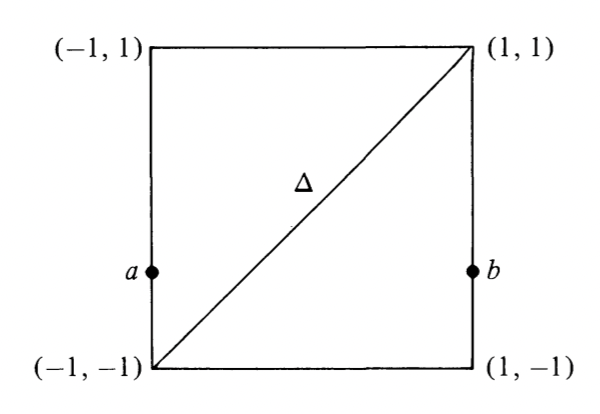
\includegraphics[width=.5\textwidth]{../images/AnIntroductionToAlgebraicTopology/1.png}
\label{}
\end{figure}
If \(G\) is the graph of \(f\) and \(\Delta\) is the graph of the identity function, then we must prove
that \(G\cap\Delta\neq\emptyset\). The idea is to use a connectness argument to show that every path in \(D^1\times D^1\)
from \(a\) to \(b\) must cross \(\Delta\).

Since \(f\) is continuous, \(G=\{(x,f(x)):x\in D^1\}\) is connected (continuous image of connected
space is connected). Define \(A=\{(x,f(x)):f(x)>x\}\)  and \(B=\{(x,f(x)):f(x)<x\}\). Note
that \(a\in A\) and \(b\in B\), so that \(A\neq\emptyset\) and \(B\neq\emptyset\). If \(G\cap\Delta=\emptyset\), then \(G\) is the disjoint
union of \(A\) and \(B\).
\end{proof}

\begin{definition}[]
A subspace \(X\) of a topological space \(Y\) is a \textbf{retract} of \(Y\) if there is a continuous
map  \(r:Y\to X\) with \(r(x)=x\) for all \(x\in X\); such a map \(r\) is called a \textbf{retraction}
\end{definition}



\begin{theorem}[Brouwer fixed point theorem]
If \(f:D^n\to D^n\) is continuous, then there exists \(x\in D^n\) with \(f(x)=x\)
\end{theorem}

\section{Categories and Functors}
\label{sec:orgae4311b}
\begin{definition}[]
A category \(\calc\) consists of three ingredients: a class of \textbf{objects}, \(\obj\calc\); sets of
\textbf{morphisms} \(\Hom(A,B)\), one for every ordered pair \(A,B\in\obj\calc\);
\textbf{composition} \(\Hom(A,B)\times\Hom(B,C)\to\Hom(A,C)\), denoted by \((f,g)\to g\circ f\), for
every \(A,B,C\in\obj\calc\) satisfying the following axioms
\begin{enumerate}
\item the family of \(\Hom(A,B)\)'s is pairwise disjoint
\item composition is associative when defined
\item for each \(A\in\obj\calc\) there exists an identity \(1_A\in\Hom(A,A)\) satisfying \(1_A\circ f=f\) for
every \(f\in\Hom(B,A)\), all \(B\in\obj\calc\) and \(g\circ 1_A=g\) for every \(g\in\Hom(A,C)\), all \(C\in\obj\calc\)
\end{enumerate}
\end{definition}

\begin{definition}[]
Let \(\calc\) and \(\cala\) be categories with \(\obj\calc\subset\obj\cala\). If \(A,B\in\obj\calc\), let's denote the two
possible Hom sets by \(\Hom_{\calc}(A,B)\) and \(\Hom_{\cala}(A,B)\). Then \(\calc\) is a \textbf{subcategory}
of \(\cala\) if \(\Hom_{\calc}(A,B)\subset\Hom_{\cala}(A,B)\) for all \(A,B\in\obj\calc\) and if composition in \(\calc\) is
the same as composition in \(\cala\)
\end{definition}

\begin{examplle}[]
\(\calc=\Top^{2}\). here \(\obj\calc\) consists of all ordered pairs \((X,A)\) where \(X\) is a topological
space and \(A\) is a subspace of \(X\). A morphism \(f:(X,A)\to(Y,B)\) is an ordered
pair \((f,f')\) where \(f:X\to Y\) is continuous and \(fi=jf'\) (where \(i\) and \(j\) are
inclusions)
\begin{center}
\begin{tikzcd}
A\arrow[r,hookrightarrow,"i"]\arrow[d,"f'"']&X\arrow[d,"f"]\\
B\arrow[r,hookrightarrow,"j"']&Y
\end{tikzcd}
\end{center}
and composition is coordinatewise. \(\Top^2\) is called the category of \textbf{pairs} (of topological spaces)
\end{examplle}

\begin{examplle}[]
\(\calc=\Top_*\). Here \(\obj\calc\) consists of all ordered pairs \((X,x_0)\) where \(X\) is a
topological space and \(x_0\) is a point of \(X\). \(\Top_*\) is a subcategory of \(\Top^2\) and
it is called the category of \textbf{pointed spaces}; \(x_0\) is called the \textbf{basepoint} of \((X,x_0)\) and
morphisms are called \textbf{pointed maps} (or \textbf{basepoint preserving maps}). The category \(\Sets_*\) of
pointed sets is defined similarly
\end{examplle}

\begin{exercise}
\label{ex0.7}
Let \(f\in\Hom(A,B)\) be a morphism in a category \(\calc\). If \(f\) has a left inverse \(g\)
(\(g\in\Hom(B,A)\)$\backslash$ and \(g\circ f=1_A\)) and a right inverse \(h\) (\(h\in\Hom(B,A)\) and \(f\circ h=1_B\)),
then \(g=h\)
\end{exercise}

\begin{exercise}
\label{ex0.9}
A set \(X\) is called \textbf{quasi-ordered} (or \textbf{pre-ordered}) if \(X\) has a transitive and reflexive
relation \(\le\) (such a set is partially ordered if \(\le\) is antisymmetric). Prove that the
following construction gives a category \(\calc\). Define \(\obj\calc=X\), if \(x,y\in X\)
and \(x\not\le y\), define \(\Hom(x,y)=\emptyset\); if \(x\le y\), define \(\Hom(x,y)\) to be a set with
exactly one element, denoted by \(i_y^x\); if \(x\le y\le z\) define composition by \(i_z^y\circ i_y^x=i_z^x\)
\end{exercise}

\begin{exercise}
\label{ex0.10}
Let \(G\) be a \textbf{monoid}, that is, a semigroup with 1. Show that the following gives a
category \(\calc\). Let \(\obj\calc\) have exactly one element, denoted by *​; define \(\Hom(*,*)=G\) and
define composition \(G\times G\to G\) as the given multiplication in \(G\)
\end{exercise}

\begin{definition}[]
A \textbf{diagram} in a category \(\calc\) is a directed graph whose vertices are labeled by objects of \(\calc\) and
whose directed edges are labeled by morphisms in \(\calc\). A \textbf{commutative diagram} in \(\calc\) is a diagram in
which, for each pair of vertices, every two paths (composites) between them are equal as
morphisms.
\end{definition}

\begin{exercise}
\label{ex0.12}
Given a category \(\calc\), shows that the following construction gives a category \(\calm\). First, an
object of \(\calm\) is a morphism of \(\calc\). Next, if \(f,g\in\obj\calm\), say \(f:A\to B\) and \(g:C\to D\),
then a morphism in \(\calm\) is an ordered pair \((h,k)\) of morphisms in \(\calc\) s.t. the diagram
\begin{center}\begin{tikzcd}
A\arrow[r,"f"]\arrow[d,"h"']&B\arrow[d,"k"]\\
C\arrow[r,"g"']&D
\end{tikzcd}\end{center}
commutes. Define composition coordinatewise
\begin{equation*}
(h',k')\circ(h,k)=(h'\circ h,k'\circ k)
\end{equation*}
\end{exercise}

\index{congruence}
\begin{definition}[]
A \textbf{congruence} on a category \(\calc\) is an equivalence relation \(\sim\) on the
class \(\bigcup_{(A,B)}\Hom(A,B)\) of all morphisms in \(\calc\) s.t.
\begin{enumerate}
\item \(f\in\Hom(A,B)\) and \(f\sim f'\) implies \(f'\in\Hom(A,B)\)
\item \(f\sim f'\), \(g\sim g'\) and the composite \(g\circ f\) exists imply that
\begin{equation*}
g\circ f\sim g'\circ f'
\end{equation*}
\end{enumerate}
\end{definition}

\begin{theorem}[]
\label{thm0.4}
Let \(\calc\) be a category with congruence \(\sim\) and let \([f]\) denote the equivalence class of a
morphism \(f\). Define \(\calc'\) as follows
\begin{align*}
\obj\calc'&=\obj\calc\\
\Hom_{\calc'}(A,B)&=\{[f]:f\in\Hom_{\calc}(A,B)\}\\
[g]\circ[f]&=[g\circ f]
\end{align*}
Then \(\calc'\) is a category
\end{theorem}

\begin{proof}
Property 1 in the definition of congruence shows that \(\sim\) partitions each set \(\Hom_{\calc}(A,B)\)
and this implies that \(\Hom_{\calc'}(A,B)\) is a set; moreover, the family of these sets is pairwise
disjoint. Property 2 in the definition of congruence shows that composition in \(\calc'\) is
well. \(\calc'\) is associative and \([1_A]\) is the identity is not hard
\end{proof}

The category \(\calc'\) is called a \textbf{quotient category} of \(\calc\); one usually
denotes \(\Hom_{\calc'}(A,B)\) by \([A,B]\)

\begin{exercise}
\label{ex0.14}
Let \(G\) be a group and let \(\calc\) be the one-object category it
defines: \(\obj\calc=\{*\}\), \(\Hom( *, *)=G\) and composition is the group operation. If \(H\) is a
normal subgroup of \(G\), define \(x\sim y\) to mean \(xy^{-1}\in H\). Show that \(\sim\) is a congruence
on \(\calc\) and that \([*, *]=G/H\) in the corresponding quotient category
\end{exercise}

\index{functor}
\begin{definition}[]
If \(\cala\) and \(\calc\) are categories, a \textbf{functor} \(T:\cala\to\calc\) is a function, that is,
\begin{enumerate}
\item \(A\in\obj\cala\) implies \(TA\in\obj\calc\)
\item if \(f:A\to A'\) is a morphism in \(\cala\), then \(Tf:TA\to TA'\) is a morphism in \(\calc\)
\item if \(f,g\) are morphisms in \(\cala\) for which \(g\circ f\) is defined, then
\begin{equation*}
T(g\circ f)=(Tg)\circ (Tf)
\end{equation*}
\item \(T(1_A)=1_{TA}\) for every \(A\in\obj\cala\)
\end{enumerate}
\end{definition}

\begin{examplle}[]
If \(\calc\) is a category, the \textbf{identity functor} \(J:\calc\to\calc\) is defined by \(JA=A\) for every
object \(A\) and \(Jf=f\) for every morphism
\end{examplle}

\begin{examplle}[]
If \(M\) is a fixed topological space, Then \(T_m:\Top\to\Top\) is a functor,
where \(T_M(X)=X\times M\) and if \(f:X\to Y\) is continuous, then \(T_M(f):X\times M\to Y\times M\) is defined by
\((x,m)\mapsto(f(x),m)\)
\end{examplle}

\begin{examplle}[]
Fix an object \(A\) in category \(\calc\). Then \(\Hom(A,-):\calc\to\Sets\) is a functor assigning to each
object \(B\) the set \(\Hom(A,B)\) and to each morphism \(f:B\to B'\) the \textbf{induced
map} \(\Hom(A,f):\Hom(A,B)\to\Hom(A,B')\) defined by \(g\mapsto f\circ g\). One usually denotes the induced
map \(\Hom(A,f)\) by \(f_*\)
\end{examplle}

Functors as just defined are also called \textbf{covariant functors} to distinguish them from
\textbf{contravariant functors} that reverse the direction of arrows. Thus the functor of the example  is
sometimes called a \textbf{covariant Hom functor}.

\begin{definition}[]
if \(\cala\) and \(\calc\) are categories, a \textbf{contravariant functor} \(S:\cala\to\calc\) is a function that
\begin{enumerate}
\item \(A\in\obj\cala\) implies \(SA\in\obj\calc\)
\item if \(f:A\to A'\) is a morphism in \(\calc\), then \(Sf:SA'\to SA\) is a morphism in \(\calc\)
\item if \(f,g\) are morphisms in \(\cala\) for which \(g\circ f\) is defined, then
\begin{equation*}
S(g\circ f)=S(f)\circ S(g)
\end{equation*}
\item \(S(1_A)=1_{SA}\) for every \(A\in\obj\cala\)
\end{enumerate}
\end{definition}

\begin{examplle}[]
Fix an object \(B\) in a category \(\calc\). Then \(\Hom(-,B):\calc\to\Sets\) is a contravariant functor
assigning to each object \(A\) the set \(\Hom(A,B)\) and to each morphism \(g:A\to A'\) the
\textbf{induced map} \(\Hom(g,B):\Hom(A',B)\to\Hom(A,B)\) defined by \(h\mapsto h\circ g\). One usually denotes the
induced map \(\Hom(g,B)\) by \(g^*\); \(\Hom(-,B)\) is called a \textbf{contravariant Hom functor}
\end{examplle}

\begin{definition}[]
An \textbf{equivalence} in a category \(\calc\) is a morphism \(f:A\to B\) for which there exists a
morphism \(g:B\to A\) with \(f\circ g=1_B\) and \(g\circ f=1_A\)
\end{definition}

\begin{theorem}[]
If \(\cala\) and \(\calc\) are categories and \(T:\cala\to\calc\) is a functor of either variance, then \(f\) an
equivalence in \(\cala\) implies that \(Tf\) is an equivalence in \(\calc\)
\end{theorem}

\begin{exercise}
\label{ex0.17}
Let \(\calc\) and \(\cala\) be categories, let \(\sim\) be a congruence on \(\calc\). If \(T:\calc\to\cala\) is a functor
with \(T(f)=T(g)\) whenever \(f\sim g\), then \(T\) defines a functor \(T':\calc'\to\cala\) (where \(\calc'\) is
the quotient category) by \(T'(X)=T(X)\) for every object \(X\) and \(T'([f])=T(f)\) for every
morphism \(f\).
\end{exercise}

\begin{exercise}
\label{ex0.20}
\begin{enumerate}
\item if \(X\) is a topological space,  show that \(C(X)\), the set of all continuous real-valued
functions on \(X\), is a commutative ring with 1 under pointwise operations
\begin{equation*}
f+g:x\mapsto f(x)+g(x)\quad\text{ and }\quad f\cdot g\mapsto f(x)g(x)
\end{equation*}
for all \(x\in X\)
\item show that \(X\mapsto C(X)\) gives a (contravariant) functor \(\Top\to\Rings\)
\end{enumerate}
\end{exercise}

\begin{proof}
\begin{enumerate}
\setcounter{enumi}{1}
\item From exercise \ref{ex0.12}
\end{enumerate}
\end{proof}


\section{Some Basic Topological Notions}
\label{sec:org6cc49e4}

\subsection{Homotopy}
\label{sec:org003f756}
\index{homotopy}
\begin{definition}[]
If \(X\) and \(Y\) are spaces and if \(f_0,f_1\) are continuous maps from \(X\) to \(Y\),
then \(f_0\) is \textbf{homotopic} to \(f_1\), denoted by \(f_0\simeq f_1\) if there is a continuous
map \(F:X\times\bI\to Y\) with
\begin{equation*}
F(x,0)=f_0(x) \quad\text{ and }\quad F(x,1)=f_1(x) \quad\text{for all }x\in X
\end{equation*}
Such a map \(F\) is called a \textbf{homotopy}, written as \(F:f_0\simeq f_1\)
\end{definition}

If \(f_t:X\to Y\) is defined by \(f_t(x)=F(x,t)\), then a homotopy \(F\) gives a one-parameter
family of continuous maps deforming \(f_0\) into \(f_1\)

\begin{lemma}[Gluing lemma]
Assume that a space \(X\) is a finite union of closed subsets \(X=\bigcup_{i=1}^nX_i\). If, for some
space \(Y\), there are continuous maps \(f_i:X_i\to Y\) that agree on overlaps
(\(f_i|X_i\cap X_j=f_j|X_i\cap X_j\) for all \(i,j\)), then there exists a unique continuous \(f:X\to Y\)
with \(f|X_i=f_i\) for all \(i\)
\end{lemma}

\begin{proof}
If \(C\) is closed in \(Y\), then
\begin{align*}
f^{-1}(C)&=X\cap f^{-1}(C)=(\bigcup X_i)\cap f^{-1}(C)\\
&=\bigcup (X_i\cap f^{-1}(C))\\
&=\bigcup (X_i\cap f_i^{-1}(C))=\bigcup f_i^{-1}(C)
\end{align*}
Since each \(f_i\) is continuous, \(f_i^{-1}(C)\) is closed in \(X_i\). Since \(X_i\) is closed
in \(X\), \(f_i^{-1}(C)\) is closed in \(X\), therefore \(f^{-1}(C)\) is closed in \(X\) and \(f\)
is continuous
\end{proof}

\begin{lemma}[Gluing Lemma]
Assume that a space \(X\) has a (possibly infinite) open cover \(X=\bigcup X_i\). If for some
space \(Y\), there are continuous maps \(f_i:X_i\to Y\) that agree on overlaps, then there exists a
unique continuous \(f:X\to Y\) with \(f|X_i=f_i\) for all \(i\)
\end{lemma}

\begin{theorem}[]
Homotopy is an equivalence relation on the set of all continuous maps \(X\to Y\)
\end{theorem}

\begin{proof}
\emph{Reflexivity}. If \(f:X\to Y\), define \(F:X\times\bI\to Y\) by \(F(x,t)=f(x)\) for all \(x\in X\) and \(t\in\bI\);
clearly \(F:f\simeq f\)

\emph{Symmetry}: Assume that \(f\simeq g\), so there is a continuous \(F:X\times\bI\to Y\) with \(F(x,0)=f(x)\)
and \(F(x,1)=g(x)\) for all \(x\in X\). Define \(G:X\times\bI\to Y\) by \(G(x,t)=F(x,1-t)\), and note
that \(G:g\simeq f\).

\emph{Transivity}: assume that \(F:f\simeq g\) and \(G:g\simeq h\). Define \(H:X\times\bI\to Y\) by
\begin{equation*}
H(x,t)=
\begin{cases}
F(x,2t)&0\le t\le 1/2\\
G(x,2t-1)&1/2\le t\le 1
\end{cases}
\end{equation*}
Because these functions agree on the overlap \(\{(x,1/2):x\in X\}\), the gluing lemma shows
that \(H\) is continuous. Therefore \(H:f\simeq h\)
\end{proof}

\begin{definition}[]
If \(f:X\to Y\) is continuous, its \textbf{homotopy class} is the equivalence class
\begin{equation*}
[f]=\{\text{continuous }g:X\to Y:g\simeq f\}
\end{equation*}
The family of all such homotopy classes is denoted by \([X,Y]\)
\end{definition}

\begin{theorem}[]
Let \(f_i:X\to Y\) and \(g_i:Y\to Z\), for \(i=0,1\), be continuous. If \(f_0\simeq f_1\) and \(g_0\simeq g_1\),
then \(g_0\circ f_0\simeq g_1\circ f_1\); that is, \([g_0\circ f_0]=[g_1\circ f_1]\)
\end{theorem}

\begin{proof}
Let \(F:f_0\simeq f_1\) and \(G:g_0\simeq g_1\) be homotopies. First, we show that
\begin{equation*}
g_0\circ f_0\simeq g_1\circ f_0
\end{equation*}
Define \(H:X\times\bI\to Z\) by \(H(x,t)=G(f_0(x),t)\). Clearly, \(H\) is continuous;
moreover, \(H(x,0)=G(f_0(x),0)=g_0(f_0(x))\) and \(H(x,1)=G(f_0(x),1)=g_1(f_0(x))\). Now observe
that
\begin{equation*}
K:g_1\circ f_0\sim g_1\circ f_1
\end{equation*}
where \(K:X\times\bI\to Z\) is the composite \(g_1\circ F\). Now use the transitivity of the homotopy relation,
we have \(g_0\circ f_0\simeq g_1\circ f_1\)
\end{proof}

\begin{corollary}[]
Homotopy is a congruence on the category \(\Top\).
\end{corollary}

It follows from Theorem \ref{thm0.4} that there is a quotient category whose objects are
topological spaces \(X\), whose Hom sets are \(\Hom(X,Y)=[X,Y]\) and whose composition
is \([g]\circ[f]=[g\circ f]\)

\begin{definition}[]
The quotient category just described is called the \textbf{homotopy category}, and it is denoted by
\(\hTop\)
\end{definition}

All the functors \(T:\Top\to\cala\) that we shall construct, where \(\cala\) is some ``algebraic'' category
(e.g. \(\Ab\), \(\Groups\), \(\Rings\)) will have the property that \(f\simeq g\)
implies \(T(f)=T(g)\). This fact, aside from a natural wish to identify homotopic maps, makes
homotopy valuable, \emph{beacause it guarantees that the algebraic problem in \(\cala\) arising from a}
\emph{topological problem via \(T\) is simpler than the original problem}

\begin{definition}[]
A continuous map \(f:X\to Y\) is a \textbf{homotopy equivalence} if there is a continuous map \(g:Y\to X\)
with \(g\circ f\simeq 1_X\) and \(f\circ g\simeq 1_Y\). Two spaces \(X\) and \(Y\) have the \textbf{same homotopy type} if
there is a homotopy equivalence \(f:X\to Y\)
\end{definition}

\(f\) is a homotopy equivalence iff \([f]\in[X,Y]\) is an equivalence in \(\hTop\). (\label{Problem1})

\begin{definition}[]
Let \(X\) and \(Y\) be spaces, and let \(y_0\in Y\). The \textbf{constant map} at \(y_0\) is the
function \(c:X\to Y\) with \(c(x)=y_0\) for all \(x\in X\). A continuous map \(f:X\to Y\) is
\textbf{nullhomotopic} if there is a constant map \(c:X\to Y\) with \(f\simeq c\)
\end{definition}

\begin{theorem}[]
\label{thm1.5}
Let \(\C\) denote the complex numbers, let \(\Sigma_\rho\subset\C\approx\R^2\) denote the circle with center at the origin
0 and radius \(\rho\), and let \(f_\rho^n:\Sigma_\rho\to\C-\{0\}\) denote the restriction to \(\Sigma^\rho\) of \(z\mapsto z^n\). If none
of the maps \(f_\rho^n\) is nullhomotopic (\(n\ge 1\) and \(\rho>0\)) then the fundamental theorem of
algebra is true (i.e., every nonconstant complex polynomial has a complex root)
\end{theorem}

\begin{proof}
Consider the polynomial with complex coefficients
\begin{equation*}
g(z)=z^n+a_{n-1}z^{n-1}+\dots+a_1z+a_0
\end{equation*}
Choose \(\rho>\max\{1,\sum_{i=1}^{n-1}\abs{a_i}\}\) and define \(F:\Sigma_\rho\times\bI\to\C\)
\begin{equation*}
F(z,t)=z^n+\sum_{i=0}^{n-1}(1-t)a_iz^i
\end{equation*}
It's obvious that \(F:g|\Sigma_\rho\simeq f_\rho^n\) if we can show that the image of \(F\) is contained
in \(\C-\{0\}\). that is, \(F(z,t)\neq0\). If, on the contrary, \(F(z,t)=0\)  for some \(t\in\bI\) and
some \(z\) with \(\abs{z}=\rho\), then \(z^n=-\sum_{i=0}^{n-1}(1-t)a_iz^i\). The triangle inequality gives
\begin{equation*}
\rho^n\le\sum_{i=0}^{n-1}(1-t)\abs{a_i}\rho^i\le\sum_{i=0}^{n-1}\abs{a_i}\rho^i\le\left(\sum_{i=0}^{n-1}\abs{a_i}\right)\rho^{n-1}
\end{equation*}
for \(\rho>1\) implies that \(\rho^i\le\rho^{n-1}\). Canceling \(\rho^{n-1}\) gives \(\rho\le\sum_{i=0}^{n-1}\abs{a_i}\),
a contradiction.

Assume now that \(g\) has no complex roots. Define \(G:\Sigma_\rho\times\bI\to\C-\{0\}\) by
\(G(z,t)=g((1-t)z)\). (Since \(g\) has no roots, the values of \(G\) do lie in \(\C-\{0\}\))
Visibly, \(G:g|\Sigma_\rho\simeq k\), where \(k\) is the constant function at \(a_0\). Therefore \(g|\Sigma_\rho\) is
nullhomotopic and by transitivity, \(f_\rho^n\) is nullhomotopic, contradicting the hypothesis.
\end{proof}

A common problem involves extending a map \(f:X\to Z\) to a larger space \(Y\); the picture is
\begin{center}\begin{tikzcd}
Y\arrow[dr,dashed,"g"]\\
X\arrow[u,hookrightarrow]\arrow[r,"f"']&Z
\end{tikzcd}\end{center}
Homotopy itself raises such a problem: if \(f_0,f_1:X\to Z\) then \(f_0\simeq f_1\) if we can
extend \(f_0\cup f_1:X\times\{0\}\cup X\times\{1\}\to Z\) to all of \(X\times\bI\)

\begin{theorem}[]
\label{thm1.6}
Let \(f:S^n\to Y\) be a continuous map into some space \(Y\). TFAE
\begin{enumerate}
\item \(f\) is nullhomotopic
\item \(f\) can be extended to a continuous map \(D^{n+1}\to Y\)
\item if \(x_0\in S^n\) and \(k:S^n\to Y\) is the constant map at \(f(x_0)\), then there is a
homotopy \(F:f\simeq k\) with \(F(x_0,t)=f(x_0)\) for all \(t\in\bI\)
\end{enumerate}
\end{theorem}

\begin{proof}
\(1\to 2\). Assume that \(F:f\simeq c\) , where \(c(x)=y_0\) for all \(x\in S^n\). Define \(g:D^{n+1}\to Y\)
by
\begin{equation*}
g(x)=
\begin{cases}
y_0&0\le\norm{x}\le 1/2\\
F(x/\norm{x},2-2\norm{x})&1/2\le\norm{x}\le 1
\end{cases}
\end{equation*}
if \(x\neq 0\), then \(x/\norm{x}\in S^n\); if \(1/2\le\norm{x}\le 1\) then \(2-2\norm{x}\in\bI\);
if \(\norm{x}=1/2\) then \(2-2\norm{x}=1\) and \(F(x/\norm{x},1)=c(x/\norm{x})=y_0\). The gluing
lemma shows that \(g\) is continuous. Finally \(g\) does extend \(f\): if \(x\in S^n\),
then \(\norm{x}=1\) and \(g(x)=F(x,0)=f(x)\).

\(2\to 3\). Assume that \(g:D^{n+1}\to Y\) extends \(f\). Define \(F:S^n\times\bI\to Y\)
by \(F(x,t)=g((1-t)x+tx_0)\); note that \((1-t)x+tx_0\in D^{n+1}\). Visibly \(F\) is continuous.
Now \(F(x,0)=g(x)=f(x)\) while \(F(x,1)=g(x_0)=f(x_0)\) for all \(x\in S^n\); hence \(F:f\simeq k\)
where \(k:S^n\to Y\) is the constant map at \(f(x_0)\). Finally, \(F(x_0,t)=g(x_0)=f(x_0)\) for
all \(t\in\bI\)

\(3\to 1\) obvious
\end{proof}

\subsection{Convexity, Contractibility, and Cones}
\label{sec:orgafeb14d}
\begin{definition}[]
A subset \(X\) of \(\R^m\) is \textbf{convex} if for each pair of points \(x,y\in X\) the line segment
joining \(x\) and \(y\) is contained in \(X\). In other words, if \(x,y\in X\),
then \(tx+(1-t)y\in X\) for all \(t\in\bI\)
\end{definition}

\begin{definition}[]
A space \(X\) is \textbf{contractible} if \(1_X\) is nullhomotopic
\end{definition}

\begin{theorem}[]
\label{thm1.7}
Every convex set \(X\) is contractible
\end{theorem}

\begin{proof}
Choose \(x_0\in X\), and define \(c:X\to X\) by \(c(x)=x_0\) for all \(x\in X\). Define \(F:X\times\bI\to X\)
by \(F(x,t)=tx_0+(1-t)x\). Hence \(F:1_X\simeq c\).
\end{proof}

A hemisphere is contractible but not convex, so that the converse of Theorem \ref{thm1.7} is not
true

\begin{exercise}
\label{ex1.3}
Let \(R:S^1\to S^1\) be rotation by \(\alpha\) radians. Prove that \(R\simeq 1_S\). Conclude that every continuous
map \(f:S^1\to S^1\) is homotopic to a continuous map \(g:S^1\to S^1\) with \(g(1)=1\)
(where \(1=e^{2\pi i0}\in S^1\))
\end{exercise}

\begin{proof}
Let \(F:S^1\times\bI\to S^1\) be
\begin{equation*}
F((\cos\theta,\sin\theta),t)=(\cos(\theta+\alpha(1-t)),\sin(\theta+\alpha(1-t)))
\end{equation*}
\end{proof}

\begin{exercise}
\label{ex1.5}
\label{Problem2}
Let \(X=\{0\}\cup\{1,1/2,1/3,\dots,1/n,\dots\}\) and let \(Y\) be a countable discrete space. Show that \(X\)
and \(Y\) do not have the same homotopy type.
\end{exercise}

\begin{definition}[]
Let \(X\) be a topological space and let \(X'=\{X_j:j\in J\}\) be a partition of \(X\). The \textbf{natural
map} \(\nu:X\to X'\) is defined by \(\nu(x)=X_j\) where \(x\in X_j\). The \textbf{quotient topology} on \(X'\) is
the family of all subsets \(U'\) of \(X'\) for which \(\nu^{-1}(U')\) is open in \(X\)
\end{definition}

\(\nu:X\to X'\) is continuous when \(X'\) has the quotient topology. There are two special cases that
we wish to mention. If \(A\) is a subset of \(X\), then we write \(X/A\) for \(X'\), where the
partition of \(X\) consists of \(A\) together with all the one-point subsets of \(X-A\). The
second special case arises from an equivalence relation \(\sim\) on \(X\).  In this case, the
partition consists of the equivalence classes, the natural map is given by \(\nu:x\mapsto[x]\), and the
quotient space is denoted by \(X/\sim\).

\begin{examplle}[]
Let \(X=\bI\times\bI\)
\begin{figure}[htbp]
\centering
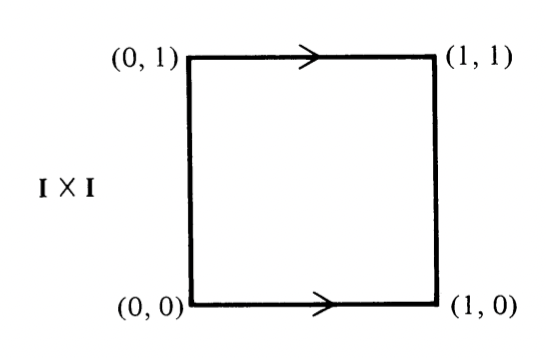
\includegraphics[width=.4\textwidth]{../images/AnIntroductionToAlgebraicTopology/2.png}
\label{}
\end{figure}
and define \((x,0)\sim(x,1)\) for every \(x\in\bI\). Then \(X/\sim\) is homeomorphic to the
cylinder \(S^1\times\bI\). Furthermore, suppose we define a second equivalence relation on \(\bI\times\bI\)
by \((x,0)\sim(x,1)\) for all \(x\in\bI\) and \((0,y)\sim(1,y)\) for all \(y\in\bI\). Then \(\bI\times\bI/\sim\) is the
\textbf{torus} \(S^1\times S^1\)
\end{examplle}

\begin{examplle}[]
\label{example1.3}
If \(h:X\to Y\) is a function, then \(\textbf{ker \textit{h}}\) is the equivalence relation on \(X\) defined
by \(x\sim x'\) if \(h(x)=h(x')\). The corresponding quotient space is denoted by \(X/\ker h\). Note
that, given \(h:X\to Y\) there always exists an injection \(\varphi:X/\ker h\to Y\) making the diagram
\begin{center}\begin{tikzcd}[column sep=small]
X\ar[rr,"h"]\ar[dr,"\nu"']&&Y\\
&X/\ker h\ar[ur,"\varphi"']
\end{tikzcd}\end{center}
namely, \(\varphi([x])=h(x)\)
\end{examplle}

\begin{definition}[]
A continuous surjection \(f:X\to Y\) is an \textbf{identification} if a subset \(U\) of \(Y\) is open
iff \(f^{-1}(U)\) is open in \(X\)
\end{definition}

\begin{examplle}[]
If \(\sim\) is an equivalence relation on \(X\)and \(X/\sim\) is given the quotient topology, then the
natural map \(\nu:X\to X/\sim\) is an identification
\end{examplle}

\begin{examplle}[]
If \(f:X\to Y\) is a continuous surjective map having a \textbf{section} (i.e., there is a continuous \(s:Y\to X\)
with \(fs=1_Y\)), then \(f\) is an identification
\end{examplle}

\begin{theorem}[]
\label{thm1.8}
Let \(f:X\to Y\) be a continuous surjection. Then \(f\) is an identification iff for all
spaces \(Z\) and all functions \(g:Y\to Z\), one has \(g\) continuous iff \(gf\) is continuous
\begin{center}\begin{tikzcd}[column sep=small]
X\ar[rr,"gf"]\ar[dr,"f"']&&Z\\
&Y\ar[ur,"g"']
\end{tikzcd}\end{center}
\end{theorem}

\begin{proof}
Assume \(f\) is an identification. If \(g\) is continuous, then \(gf\) is continuous. Conversely,
if \(f\) is continuous and let \(V\)  be open in \(Z\). Then \(f^{-1}g^{-1}(V)\) is open
in \(X\); since \(f\) is an identification, \(g^{-1}(V)\) is open in \(Y\)

Assume the condition. Let \(Z/\ker f\), let \(\nu:X\to X/\ker f\) be the natural map and
let \(\varphi:X/\ker f\to Y\) be the injection of Example \ref{example1.3}. Note that \(\varphi\) is surjective
because \(f\) is. Consider the commutative diagram
\begin{center}\begin{tikzcd} [column sep=small]
X\ar[rr,"\nu"]\ar[rd,"f"']&&X/\ker f\\
&Y\ar[ur,"\varphi^{-1}"']
\end{tikzcd}\end{center}
Then \(\varphi^{-1}f=\nu\) is continuous implies that \(\varphi^{-1}\) is continuous, by hypothesis. Also
\(\varphi\) is continuous because \(\nu\) is an identification. We conclude that \(\varphi\) is a homeomorphism
\end{proof}

\begin{definition}[]
Let \(f:X\to Y\) be a function and let \(y\in Y\). Then \(f^{-1}(y)\) is called the \textbf{fiber} over \(y\)
\end{definition}

\begin{corollary}[]
\label{cor1.9}
Let \(f:X\to Y\) be an identification and, for some space \(Z\), let \(h:X\to Z\) be a continuous
function that is constant on each fiber of \(f\). Then \(hf^{-1}:Y\to Z\) is continuous
\begin{center}\begin{tikzcd}[column sep=small]
X\ar[rr,"h"]\ar[dr,"f"']&&Z\\
&Y\ar[ur,"hf^{-1}"']
\end{tikzcd}\end{center}
Moreover, \(hf^{-1}\) is an open (closed) map iff \(h(U)\) is open (closed) in \(Z\)
whenever \(U\) is an open (closed ) set in \(X\) of the form \(U=f^{-1}f(U)\)
\end{corollary}

\begin{proof}
\(h\) is constant on each fiber of \(f\) implies that \(hf^{-1}\) is well-defined. \(hf^{-1}\) is
continuous because \((hf^{-1})(f)=h\) is continuous, and Theorem \ref{thm1.8} applies. Finally
if \(V\) is open in \(Y\), then \(f^{-1}(V)\) is an open set of the stated form \(f^{-1}(V)=f^{-1}f(f^{-1}(V))\)
\end{proof}

\begin{corollary}[]
Let \(X\) and \(Z\) be spaces and let \(h:X\to Z\) be an identification. Then the
map \(\varphi:X/\ker h\to Z\) defined by \([x]\mapsto h(x)\) is a homeomorphism
\end{corollary}

\begin{proof}
\(\varphi\) is a bijection. \(\varphi\) is continuous by Corollary \ref{cor1.9}. The \(\nu:X\to X/\ker h\) be the natural
map. Let \(U\) open in \(X/\ker h\). Then \(h^{-1}\varphi(U)=\nu^{-1}(U)\) is an open set in \(X\),
because \(\nu\) is continuous and hence \(\varphi(U)\) is open, because \(h\) is an identification
\end{proof}
​
\section{Problem}
\label{sec:org8d2d4fd}
\label{Problem1}

\label{Problem2}

\section{Index}
\label{sec:org13604c8}
\renewcommand{\indexname}{}
\printindex
\end{document}
